\section{DC Servomotor}\label{sec:servo_motor}

The control of both antennas requires the use of two motors which will be able to change its orientation. In this project, the DC servomotor was chosen because it can be either a rotary or a linear actuator which allows a precise control of angular or linear position, velocity and acceleration.

The servomotor can be described in two different parts: an electrical motor and a servomechanism. The electrical motor is a DC motor which is able to convert electrical power into mechanical power. The shaft of the DC motor is coupled with another shaft denominated output shaft. The connection is made through a gear assembly which is not only responsible for the connection between both shafts, but also for the reduction of the RPM of the motor’s shaft (figure \ref{servomotor_expl1}).

\begin{figure}[H]
\centering
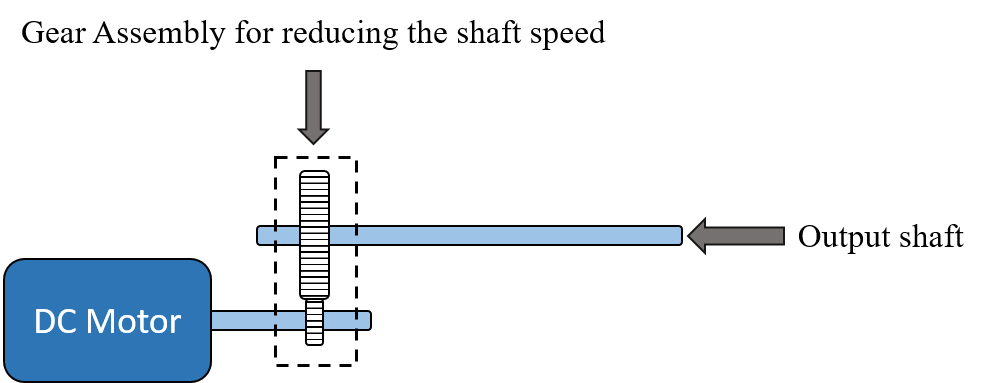
\includegraphics[scale=0.7]{figures/servomotor_expl1.png}
\caption{Connection between the output shaft and the DC motor}
\label{servomotor_expl1}
\end{figure}

The output shaft is also connected with a potentiometer by another gear assembly and, during its rotation, the knob rotates and creates an electrical signal. This signal increases proportionally with the angular movement of the potentiometer knob. The connection between the output shaft and the potentiometer can be
observer in the figure \ref{servomotor_expl2}.

\begin{figure}[H]
\centering
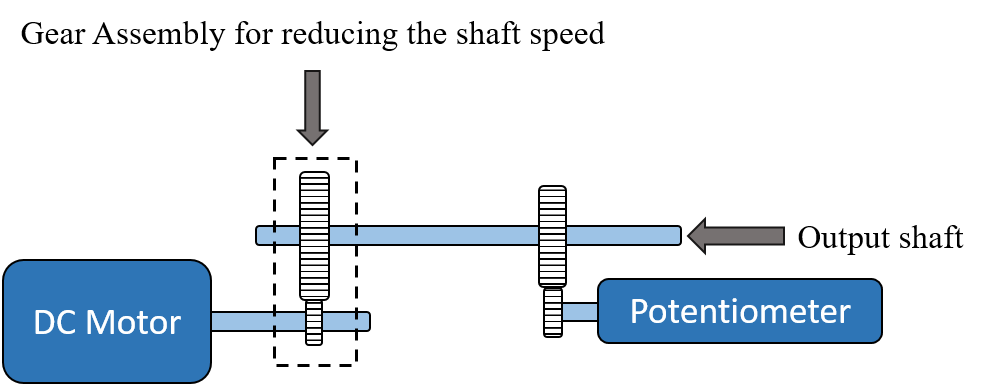
\includegraphics[scale=0.7]{figures/servomotor_expl2.png}
\caption{Connection between the output shaft and the potentiometer}
\label{servomotor_expl2}
\end{figure}

The previous described gears are involved in the gear mechanism which is responsible for the transformation of the original input speed provided by the DC motor into a slower output speed which is practical and widely applicable. 

The potentiometer is also connected with an error detector feedback amplifier where the electrical potential (from the potentiometer) and the input command voltage (the signal that represents the desired angle) are compared. The output of the error detector amplifier is called electrical input of the DC motor and is represented in the figure \ref{servomotor_expl3}. When the electrical potential equals the input voltage, which means that the shaft is in the desired position, the input of the DC motor becomes zero and the motor stops rotating until the next command.

\begin{figure}[H]
\centering
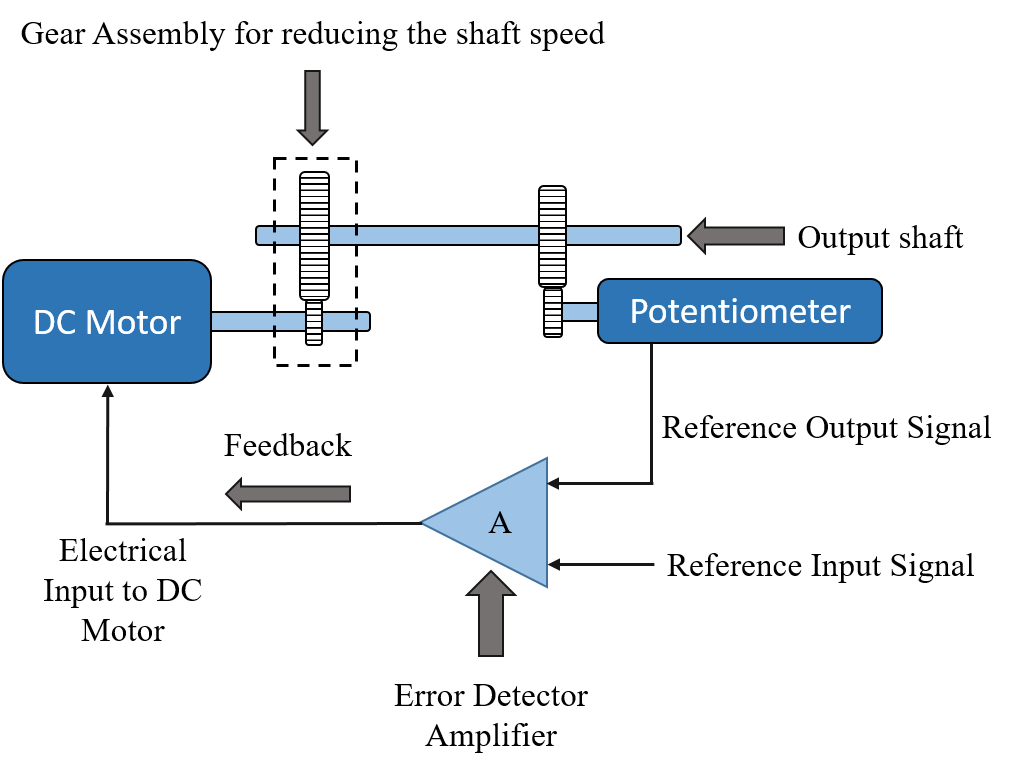
\includegraphics[scale=0.7]{figures/servomotor_expl3.png}
\caption{Servomotor’s feedback}
\label{servomotor_expl3}
\end{figure}

In order to be able to do the previous procedure it is necessary to apply a restricted input voltage signal in regular intervals. Servomotors operate from 4.8V to a 6V supply voltage, but 5V is the typical value. On the other hand, the pulse should have a specific width (PWM – Pulse Width Modulation) because it will be responsible for the amount of rotation. Typically, the duration of the pulse varies from 0ms to 2.2ms and the frequency from 50Hz to 60Hz. The size of the pulse will result in a lesser or greater rotation. The figure \ref{signal_servo} is an example of the relation pulse-rotation and describes three different cases. For instance, if the duration of the pulse is 1.25ms, the servomotor will rotate 90 degrees.

\begin{figure}[H]
\centering
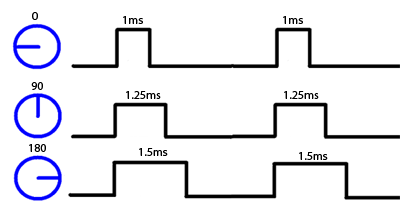
\includegraphics[scale=0.5]{figures/signal_servo.jpg}
\caption{Examples of the relation between the PWM and the rotation}
\label{signal_servo}
\end{figure}

Based on the previous explanation, the servomotor requires a power supply unit and the information about the rotation that should be done through an electrical signal. Hence, this motor needs three different terminals (the figure \ref{cable_servo} is one example of the terminals of a servo motor):
\begin{itemize}  
        \item Orange - Position signal (PWM pulses).
        \item Brown - $V_{cc}$ (from the power supply unit). 
        \item Red - Ground.
\end{itemize}

\begin{figure}[H]
\centering
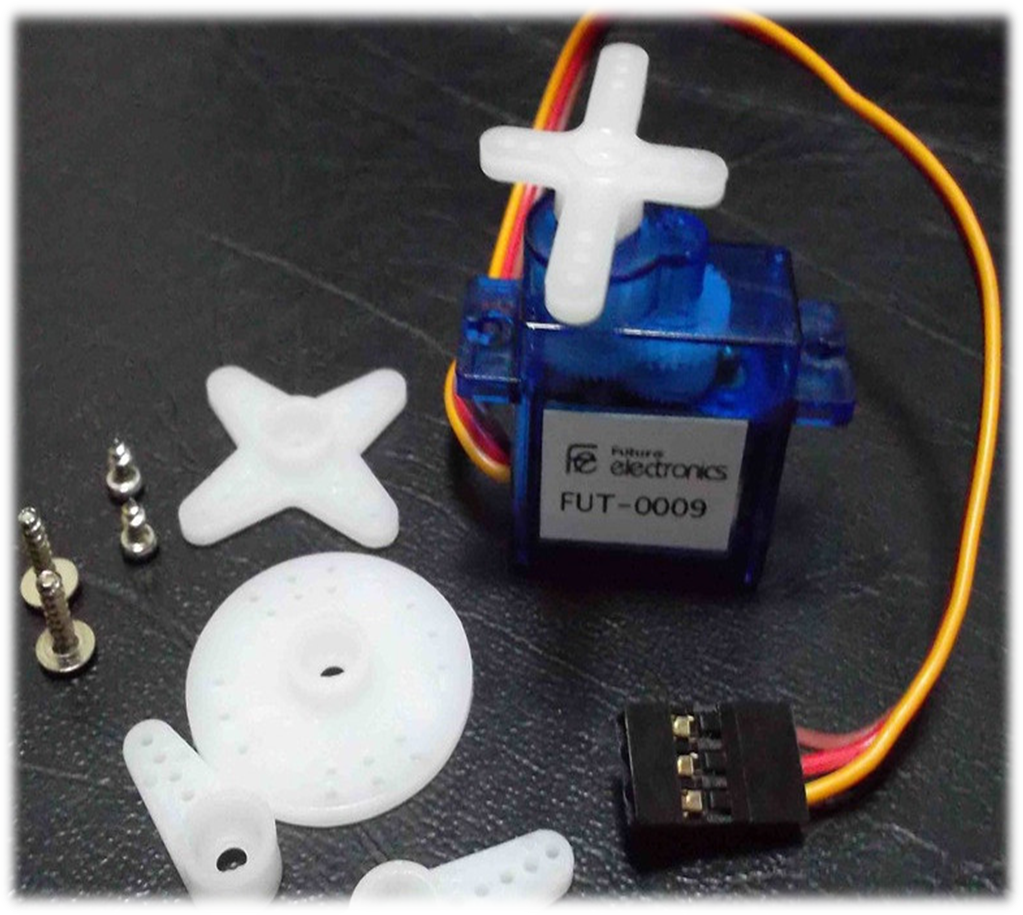
\includegraphics[scale=0.5]{figures/cable_servo.png}
\caption{Servo motor with its three different terminals}
\label{cable_servo}
\end{figure}

ANOTHER SECTION ANOTHER SECTION ANOTHER SECTION - DOESN’T MAKE SENSE HERE!!!!!!!!!!!!!!!!!

\subsection{Modelling}

As was presented before, the servomotor can be divided in two different groups: the DC motor and the servomechanism.

DC motor is an actuator which converts electrical energy to mechanical rotation. In the figure \ref{dcmotor_circuit} it is possible to see the model of this motor. DC motors are a type of motors which were built to receive a voltage as an input and, after converting this voltage, to apply a specific velocity on its shaft. In other words, DC motors are able to control the velocity of the shaft.

\begin{figure}[H]
\centering
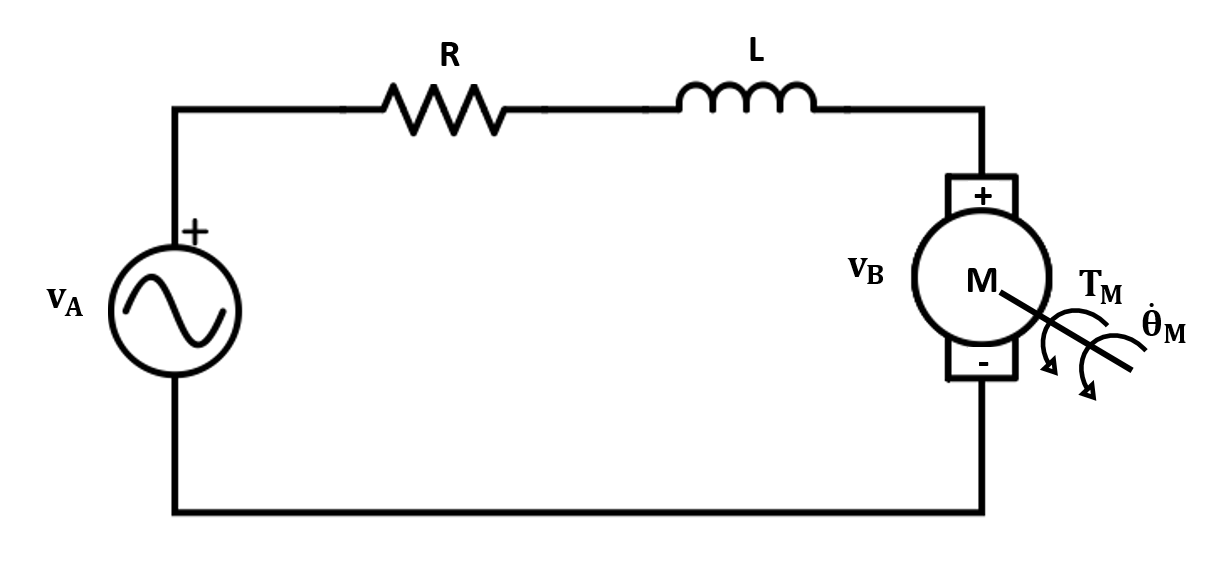
\includegraphics[scale=0.5]{figures/dcmotor_circuit.png}
\caption{Circuit of the DC motor}
\label{dcmotor_circuit}
\end{figure}

The circuit of the previous figure is described by the equations \ref{DC_motor_equation1}, \ref{DC_motor_equation2} and \ref{DC_motor_equation3}. It is possible to observe that between the source unit and the motor there are two elements (resistance and inductance). These elements are important due to the fact that they are the responsible for the stability of the system, avoiding a motor overload. On the other hand, the relation between the current and the difference between the voltage of the source and the one of the motor is made through an admitance.

\begin{equation}\label{DC_motor_equation1}
v_{a}= v_{b}+i_{a} R_{a}+L_{a}\frac{\mathrm{d} i_{a}}{\mathrm{d} t}
\end{equation}

\begin{equation}\label{DC_motor_equation2}
V_{a}(s)= V_{b}(s)+I_{a}(s) R_{a}+sL_{a}I_{a}(s)
\end{equation}

\begin{equation}\label{DC_motor_equation3}
I_{a}(s)= \frac{V_{a}(s)-V_{b}(s)}{R_{a}+sL_{a}} , I_{a}(s)= G_{I}(V_{a}(s)-V_{b}(s))
\end{equation}

The model of the figure \ref{model1} is the representation of the equation \ref{DC_motor_equation3}.

\begin{figure}[H]
\centering
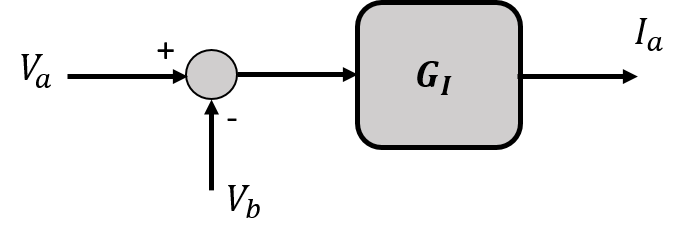
\includegraphics[scale=0.6]{figures/model1.png}
\caption{Relation between the input and the feedback voltage and the current of the circuit}
\label{model1}
\end{figure}

Furthermore, the sum of torques applied on the motor depends on the load attached to the motor shaft. The inertial and damping behaviours of the load can be represented as a inertia coefficient, $J_{e}$, and a viscous damping coefficient, $D_{e}$. This total tendency of a force to rotate an object about an axis is represented by $T_{m}$ which is described through the equation \ref{torque_time}. 

\begin{equation}\label{torque_time}
T_{m}(t)= J_{e}\frac{\mathrm{d} \dot{\theta}_{m}(t)}{\mathrm{d} t}+D_{e}\dot{\theta}_{m}(t)
\end{equation}

However, the servomotor is a type of motor which is able to control the position of the shaft. Using a potentiometer it is possible to send an electrical signal with the information about the angle. Thus, using the relation between the velocity and the position described in the equation \ref{theta_relation}, it is possible to write the equation \ref{torque_frequency_theta}.

\begin{equation}\label{theta_relation}
\dot{\theta}_{m}(s)= s\theta_{m}(s)
\end{equation}

\begin{equation}\label{torque_frequency_theta}
T_{m}(s)= (s^{2}J_{e} + sD_{e})\theta_{m}(s)
\end{equation}

The torque is also proportional to the current that passes through the circuit. The constant of proportionality is called torque constant and the relation between the torque and the current is presented in the equations \ref{torque_curr1} and \ref{torque_curr2}.

\begin{equation}\label{torque_curr1}
T_{m}(t)= K_{t} i_{a}(t)
\end{equation}

\begin{equation}\label{torque_curr2}
T_{m}(s)= K_{t} I_{a}(s)
\end{equation}

Based on the previous equations and on the model in the figure \ref{model1} it is possible to build the model in the figure \ref{model2}.

\begin{figure}[H]
\centering
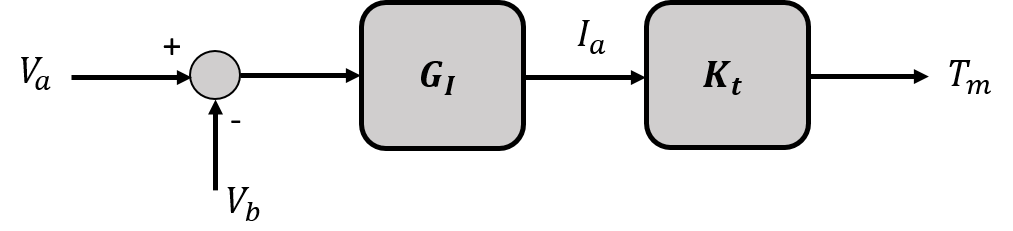
\includegraphics[scale=0.6]{figures/model2.png}
\caption{Relation between the voltage and the applied torque}
\label{model2}
\end{figure}

The applied torque $T_{m}(s)$ described in the previous equations can be also related to the angle position $\theta_{m}(s)$ through the equations \ref{torque_frequency} and \ref{torque_frequency_G}.

\begin{equation}\label{torque_frequency}
T_{m}(s) I_{a}(s)= (s^{2}J_{e} + sD_{e})\theta_{m}(s)
\end{equation}

\begin{equation}\label{torque_frequency_G}
\theta_{m}(s)= G_{\theta}(s)\times T_{m}(s) , G_{\theta}(s)=\frac{1}{s^{2}J_{e} + sD_{e}}
\end{equation}

\begin{figure}[H]
\centering
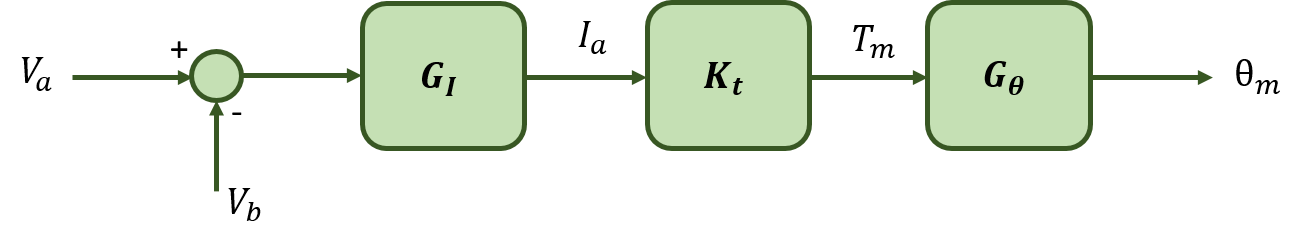
\includegraphics[scale=0.6]{figures/model3.png}
\caption{Relation between the voltage and the angle of the shaft}
\label{model3}
\end{figure}

Finally, it is also possible to calculate the relation between the output theta and voltage. Thus, the comparison between the output and the input voltage allows the formation of a closed loop using a feedback (figure \ref{model4}).

\begin{equation}\label{feedback1}
v_{b}(t)= K_{b}\frac{\mathrm{d} \theta_{m}(t)}{\mathrm{d} t}
\end{equation}

\begin{equation}\label{feedback2}
V_{b}(s)= sK_{b}\theta_{m}(s)
\end{equation}

\begin{figure}[H]
\centering
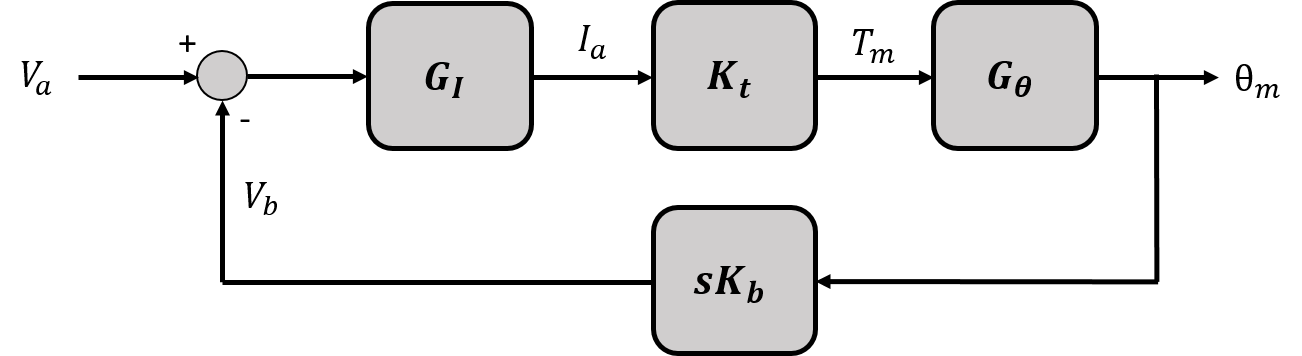
\includegraphics[scale=0.6]{figures/model4.png}
\caption{Model of a servomotor}
\label{model4}
\end{figure}